\documentclass{llncs}
\usepackage{hyperref}
\usepackage{graphicx}
\usepackage{multirow}
\graphicspath{ {images/} }
\setlength{\tabcolsep}{20pt}
\begin{document}
\title{Comparison between the Twitter Search Network and Facebook Like/Comment
Network for two Movies: The Hobbit and The Interview}
\author{Georgiana Diana Ciocirdel}
\institute{Polytechnic University of Bucharest, Romania}
\maketitle
%
\begin{abstract}
We are hereby analysing four different networks, from two social media portals,
Twitter and Facebook. The networks are related to the movies
\href{http://www.thehobbit.com/}{The Hobbit} and
\href{http://www.theinterview-movie.com/}{The Interview}. The movie The Hobbit
first appeared on the 12/01/2014 in the UK and in the month that followed in the
rest of the world. The movie ‘The Interview’ is quite controversial and has
faced many issues before being released solely in the US, first on the
12/11/2014 and then during Christmas time. We have run our analysis on data
collected around the release dates. The Twitter networks we are analysing are
directed, with edges linking users that have authored a post to users that have
retweeted it. The Facebook networks are being analysed in three consecutive
steps, marking important release dates around the world of the two movies; these
are unimodal, undirected networks, with edges linking users that have liked or
commented on the same post made by the official Facebook pages of the two
movies. The analysis reveals a few important things about the four networks: the
two Twitter networks differ a lot between them - although big, The Interview's
Twitter graph is a "young" one, meaning that authorities and hubs haven't yet
been formed properly, the posts are sparse and with very few users retweeting
more than one post. In comparison, The Hobbit's Twitter graph has well defined
authorities and most of its users have retweeted more than one popular tweet.
The Facebook networks also differ: The Hobbit has more users liking and
commenting on their posts, especially around the US release, while The Interview
network is smaller and doesn't change much in time.
\end{abstract}
%
\section{Collecting the Data}
In order to collect the necessary data for our study, we first tried to use
popular data retrieving tools, such as Wolfram Mathematica, NameGenWeb or Social
Network Importer for Node XL, but due to some Twitter
\href{https://dev.twitter.com/rest/public/rate-limiting}{rate limitations} or
malfunctioning of the tools, we resumed to writing small python scripts with the
use of the \href{https://github.com/bear/python-twitter}{Bear Python-Twitter
API}, an open-source library that provides a "pure Python interface for the
\href{https://dev.twitter.com/rest/public}{Twitter API}" and
\href{http://nodexl.codeplex.com/}{Node XL} 1.9.2 for
the Facebook queries. Due to the afore mentioned Twitter rate limitations, we
were able to query posts from 12/22/2014 to 12/29/2014 only for both movies (as
work on this project has been carried out between December 30 and 31st 2014).
Tweets can be either recent, popular or mixed, but we queried only the
popular tweets, as it would get us data about more influential users. We then
queried for the retweeters of each of the popular tweets. We collected the data
in a \href{https://gephi.org/users/supported-graph-formats/gdf-format/}{gdf file
format} and created a node for each user that has retweeted a popular tweet and
a node for each user that authored a popular tweet. We then added an edge
between each user who has retweeted a tweet and each user that had authored the
specific tweet. The Facebook data was easier to collect and we gathered
information as follows:
\begin{enumerate}
\item for The Hobbit we collected data from between:
    \begin{enumerate}
    \item 12/01/2014-12/02/2014, which marked the release dates in the UK and
        France for the London and Paris premieres;
    \item 12/04/2014-12/09/2014, which marked the release dates in the USA for
        the New York and Los Angeles premieres;
    \end{enumerate}
\item for The Interview we collected data from between:
    \begin{enumerate}
    \item 12/11/2014, which marked the Los Angeles premiere in the USA;
    \item 12/24/2014, which marked the internet release in the USA;
    \item 12/25/2014-12/26/2014, which marked the release date in the rest of
        the USA.
    \end{enumerate}
\end{enumerate}

In the resulting \href{http://graphml.graphdrawing.org/}{graphml} files, we have
created a node for each user that has liked a post or commented on a post on the
specific Facebook page. We then added an edge between each user who has
liked/commented on posts on the page.
%
\section{Facebook and Twitter Network Analysis}
In this part we are going to analyse the four networks formed with the data we
have retrieved as presented in the previous part.
%
\subsection{The Network Structure}
The two Facebook networks were taken from the official Facebook pages of the two
movies, The Hobbit and The Interview. Each node represents a user and the
links between two users are formed when both have liked or commented on the same
post made by the page. Therefore, this is an undirected network.

The two Twitter networks were formed from the search results using the queries
"the hobbit" and "the interview". We have considered the most popular posts,
i.e. the "trending topics". We have added a node to the network for each user
that has either posted or retweeted a post and then added a directed edge from
the user that has authored the tweet (the source) to the user that has retweeted
it (the target). Therefore, this is a directed network.

In this section we will analyse the four networks by interpreting the visual
layouts (the graph representation) and by combining certain metrics so as to
obtain a mathematical insight into the data. For the visual representation of
the networks, we have used \href{https://gephi.org/}{Gephi}.
%
\subsection{The Interview - the Twitter Network}
\subsubsection{Raw Results}
\begin{center}
    \begin{tabular}{ l | c }
        \hline
        \textit{Metric} & \textit{Value} \\ \hline
        Network Type & Directed \\ \hline
        Number of Nodes & 7 872 \\ \hline
        Number of Edges & 8 152 \\ \hline
        Average Degree & 1.036 \\ \hline
        Network Density & 0 \\ \hline
        Diameter & 2 \\ \hline
        Connected Components & 13 \\
        \hline
    \end{tabular}
\end{center}
%
\subsubsection{Betweenness Centrality}
We have used the
\href{https://github.com/gephi/gephi/wiki/Fruchterman-Reingold}{Fruchterman-Reingold
algorithm} in order to produce a nice visual network of all the data we have
gathered from Twitter. Then, we have enlarged the nodes with the highest
betweenness centrality in the undirected network
(\ref{fig:interview-twitter-betweennes-centrality}). This measures how often a
node appears on shortest paths between other nodes in the network, in other
words this highlights the Twitter users that have the greatest number of
retweets or the Twitter users that get their tweets retweeted in cascade. We can
easily notice how certain areas are denser than others - these are popular
tweets that have been retweeted by many other users, so the central node points
to many other nodes. There are many people who have retweeted one popular tweet,
but there aren't many people who have retweeted many popular tweets.

Unsurprisingly, the nodes with the greatest betweenness centrality correspond to
users like Seth Rogen and James Franco (who play the main characters in the
movie), The Interview (the official Twitter user of the movie),
\href{http://www.hollywoodreporter.com/}{Hollywood Reporter} (an American media
publication) or \href{www.variety.com}{Variety}, (an American magazine).
%
\begin{figure}
\centering
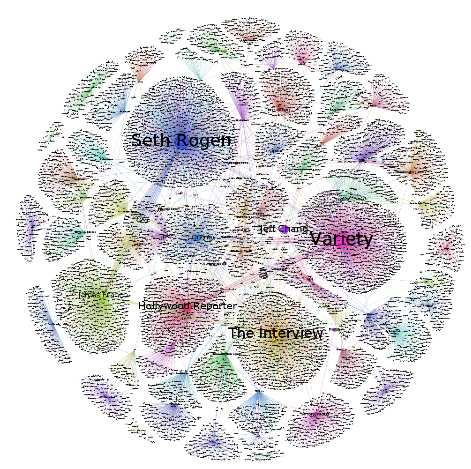
\includegraphics[width=0.6\textwidth]{interview-twitter-betweennes-centrality.png}
\caption{Highest betweenness centrality in the Fruchterman-Reingold layout for
the Twitter network of The Interview
\label{fig:interview-twitter-betweennes-centrality}}
\end{figure}
%
\subsubsection{Communities in the Network}
A community on Twitter could be
defined as a set of users that have more links within the set than outside of
it, in other words, users that share quite similar views or prefer similar
tweets and therefore, retweet them. Figure
\ref{fig:interview-twitter-communities} shows the network colored based
on different communities and the users with the highest numbers of followers
have been enlarged. These results have been yielded when determining communities
with a 20.0 modularity (we wanted to highlight only the most important
communities).
%
\begin{figure}
\centering
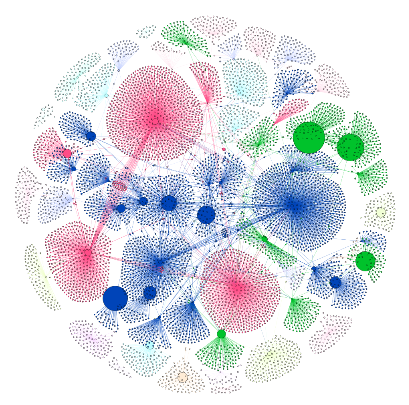
\includegraphics[width=0.6\textwidth]{interview-twitter-communities.png}
\caption{Communities in the Fruchterman-Reingold layout for the Twitter network
    of The Interview
\label{fig:interview-twitter-communities}}
\end{figure}
%
We can see from these layouts that the communities are rather fuzzy and
intertwined, but a very important thing that can be deducted is the fact that
one or more users with a huge number of followers (influential users) are part
of each of the biggest communities highlighted (the pink, the blue or the green
community). Moreover, we can now clearly see how the ideas are spread from one
small group to the other: there are users that retweet one tweet in their small
group; one of the retweeters also gets retweeted by one other user, which then
gets retweeted by many other users in his/her small group. This is, in fact, the
way the Twitter network functions.
%
\subsection{The Interview - the Facebook Network}
\subsubsection{Raw Results}
\begin{center}
    \begin{tabular}{ l | c | c }
        \hline
        \textit{Metric} & \textit{Network} & \textit{Value} \\ \hline
        \multirow{3}{*}{Network Type} & 12/11-12/2014 & Undirected \\
                                      & 12/24/2014 & Undirected \\
                                      & 12/25-26/2014 & Undirected \\ \hline
        \multirow{3}{*}{Number of Nodes} & 12/11-12/2014 & 301 \\
                                      & 12/24/2014 & 263 \\
                                      & 12/25-26/2014 & 388 \\ \hline
        \multirow{3}{*}{Number of Edges} & 12/11-12/2014 & 7 742 \\
                                      & 12/24/2014 & 6 689 \\
                                      & 12/25-26/2014 & 10 609 \\ \hline
        \multirow{3}{*}{Average Degree} & 12/11-12/2014 & 51.442 \\
                                      & 12/24/2014 & 50.87 \\
                                      & 12/25-26/2014 & 54.686 \\ \hline
        \multirow{3}{*}{Network Density} & 12/11-12/2014 & 0.171 \\
                                      & 12/24/2014 & 0.194 \\
                                      & 12/25-26/2014 & 0.141 \\ \hline
        \multirow{3}{*}{Diameter} & 12/11-12/2014 & 4 \\
                                      & 12/24/2014 & 2 \\
                                      & 12/25-26/2014 & 4 \\ \hline
        \multirow{3}{*}{Connected Components} & 12/11-12/2014 & 1 \\
                                      & 12/24/2014 & 3 \\
                                      & 12/25-26/2014 & 2 \\ \hline
    \end{tabular}
\end{center}
%
\subsubsection{Betweenness Centrality}
We have used the
\href{https://github.com/gephi/gephi/wiki/Fruchterman-Reingold}{Fruchterman-Reingold
algorithm} in order to produce a nice visual network of all the data we have
gathered from Twitter. Then, we have enlarged the nodes with the highest
betweenness centrality in the undirected network
(\ref{fig:interview-facebook-betweennes-centrality}). For the Facebook network
this shows the users that have liked or commented on more than one post in the
same day, so users who are “brokers” between two or more clusters in the
network.

One can easily notice that there is no major difference between the three
instances of the network. In all cases, there are users who have liked more than
one post and users who have liked only one, so the bigger nodes represent
“brokers” between the communities that have formed around each post.
%
\begin{figure}
\centering
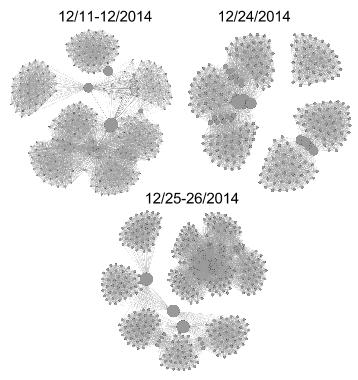
\includegraphics[width=0.6\textwidth]{interview-facebook-betweennes-centrality.jpg}
\caption{Highest betweenness centrality in the Fruchterman-Reingold layout for
    the Facebook network of The Interview
\label{fig:interview-facebook-betweennes-centrality}}
\end{figure}
%
\subsubsection{Communities in the Network}
A community on the Facebook page of the movie could be defined as a set of users
that have liked or shared one or more similar posts. Figure
\ref{fig:interview-facebook-communities} shows the
network colored based on different communities and the users with the highest
betweenness centrality have been enlarged. These results have been yielded when
determining communities with a 1.0 modularity.
%
\begin{figure}
\centering
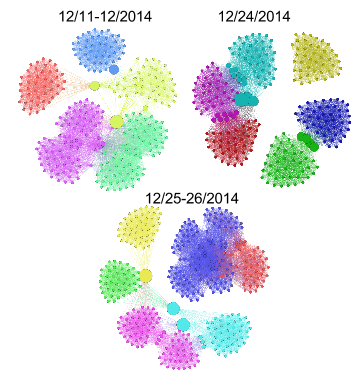
\includegraphics[width=0.6\textwidth]{interview-facebook-communities.png}
\caption{Communities in the Fruchterman-Reingold layout for the Facebook network
    of The Interview
\label{fig:interview-facebook-communities}}
\end{figure}
%
We can see from these layouts that the communities are very well defined and
very well separated from one another. It would make sense to assume that one
user who has liked the Facebook page of the movie and has then liked or
commented on a post, has maybe received the post on their timeline or has
browsed through the page's previous posts. It would also make sense to assume
that someone who has liked one post might have liked at least another one, but
if we look at the diagrams, it is clear that there aren't many users who have
done this (there aren't many brokers in the network). This could be the
consequence of the manner in which the Facebook timeline shows the posts (it
doesn't often show two updates of the same page in a row) or simply because one
page cannot publish that many important notes per day (or during a two-day
timeline).
%
\subsubsection{Connected Components}
The connected components are displayed in figure
\ref{fig:interview-facebook-cc}. The network obtained between the 11th and the
12th presents only one connected component. This might suggest that the page's
posts were all very interesting and/or important, so there were people who have
liked or commented on more than one.
%
\begin{figure}
\centering
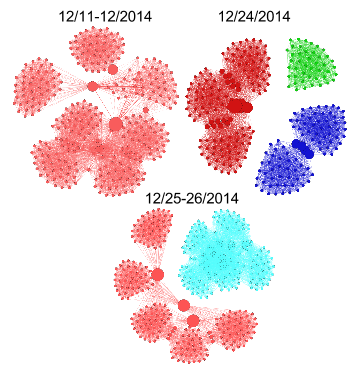
\includegraphics[width=0.7\textwidth]{interview-facebook-cc.png}
\caption{Connected components in the Fruchterman-Reingold layout for the
    Facebook network of The Interview
\label{fig:interview-facebook-cc}}
\end{figure}
%
\subsection{The Hobbit - the Twitter Network}
\subsubsection{Raw Results}
\begin{center}
    \begin{tabular}{ l | c }
        \hline
        \textit{Metric} & \textit{Value} \\ \hline
        Network Type & Directed \\ \hline
        Number of Nodes & 2 646 \\ \hline
        Number of Edges & 2 908 \\ \hline
        Average Degree & 1.099 \\ \hline
        Network Density & 0 \\ \hline
        Diameter & 2 \\ \hline
        Connected Components & 5 \\
        \hline
    \end{tabular}
\end{center}
%
\subsubsection{Betweenness Centrality}
We have again used the Fruchterman-Reingold Algorithm in order to produce a nice
visual network of all the data we have gathered from Twitter. Figure
\ref{fig:hobbit-twitter-betweennes-centrality} shows the Fruchterman-Reingold
layout of the directed Twitter network. The nodes with the highest betweenness
centrality have been enlarged. This Twitter network has a similar visual
structure as the previous one. We can easily see on the margin of the circle
users whose posts get retweeted only once. However, in the center of the circle,
there is quite a dense network of users that got their tweets shared multiple
times in a row.
%
\begin{figure}
\centering
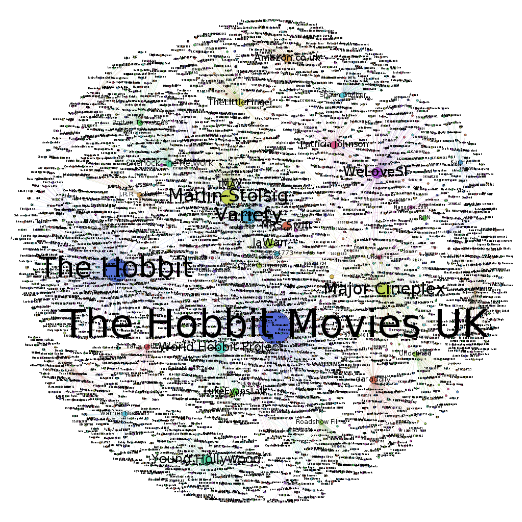
\includegraphics[width=0.7\textwidth]{hobbit-twitter-betweennes-centrality.png}
\caption{Highest betweenness centrality in the Fruchterman-Reingold layout for
the Twitter network of The Hobbit
\label{fig:hobbit-twitter-betweennes-centrality}}
\end{figure}
%
The nodes with the greatest betweenness centrality correspond to users like The
Hobbit Movies UK, The Hobbit, Major Cineplex (an operator of movie theaters in
Thailand) again the Variety magazine and a user named Marlin Stolsig, which we
could not identify. Unlike the Twitter network of 'The Interview', the most
popular users in this network are spread across the world and are not only
localized in the US.
%
\subsubsection{Communities in the Network}
Figure \ref{fig:hobbit-twitter-communities} shows the network colored based on
different communities and the users with the highest numbers of followers have
been enlarged. These results have been yielded when determining communities with
a 20.0 modularity (we wanted to highlight only the most important communities).
%
\begin{figure}
\centering
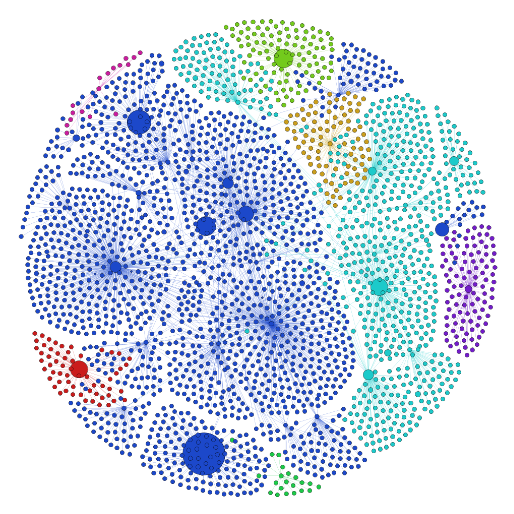
\includegraphics[width=0.8\textwidth]{hobbit-twitter-communities.png}
\caption{Communities in the Fruchterman-Reingold layout for the Twitter network
    of The Hobbit
\label{fig:hobbit-twitter-communities}}
\end{figure}
%
\subsection{The Hobbit - the Facebook Network}
\subsubsection{Raw Results}
\begin{center}
    \begin{tabular}{ l | c | c }
        \hline
        \textit{Metric} & \textit{Network} & \textit{Value} \\ \hline
        \multirow{3}{*}{Network Type} & 12/01-02/2014 & Undirected \\
                                      & 12/04-09/2014 & Undirected \\
                                      & 12/10-12/2014 & Undirected \\ \hline
        \multirow{3}{*}{Number of Nodes} & 12/01-02/2014 & 468 \\
                                      & 12/04-09/2014 & 854 \\
                                      & 12/10-12/2014 & 290 \\ \hline
        \multirow{3}{*}{Number of Edges} & 12/01-02/2014 & 12 299 \\
                                      & 12/04-09/2014 & 23 251 \\
                                      & 12/10-12/2014 & 7 110 \\ \hline
        \multirow{3}{*}{Average Degree} & 12/01-02/2014 & 52.56 \\
                                      & 12/04-09/2014 & 54.452 \\
                                      & 12/10-12/2014 & 49.034 \\ \hline
        \multirow{3}{*}{Network Density} & 12/01-02/2014 & 0.113 \\
                                      & 12/04-09/2014 & 0.046 \\
                                      & 12/10-12/2014 & 0.17 \\ \hline
        \multirow{3}{*}{Diameter} & 12/01-02/2014 & 3 \\
                                      & 12/04-09/2014 & 5 \\
                                      & 12/10-12/2014 & 2 \\ \hline
        \multirow{3}{*}{Connected Components} & 12/01-02/2014 & 5 \\
                                      & 12/04-09/2014 & 2 \\
                                      & 12/10-12/2014 & 3 \\ \hline
    \end{tabular}
\end{center}
%
\subsubsection{Betweenness Centrality}
We have used the Fruchterman-Reingold Algorithm so as to produce a visual
representation of the network in time. Figure
\ref{fig:hobbit-facebook-betweennes-centrality} shows the Fruchterman-Reingold
layout of the undirected Facebook network. As both the metrics and the
visualizations suggest, the three instances of the network are different from
one another: we can see that the first two networks are more “connected” than
the last one, meaning that in the first two networks (and more in the second
than in the first), there are many users who have liked or commented on more
than one post, so the clusters that have formed around each post are linked to
one another. Let us not forget that the movie has premiered in London and Paris
on the 1st and 2nd of December, then during the 4th and 9th it has premiered in
the US and between the 10th and 12th it has been released in other parts of
Europe. The three networks built around these dates might suggest that The
Hobbit was more popular in the US than in Europe.
%
\begin{figure}
\centering
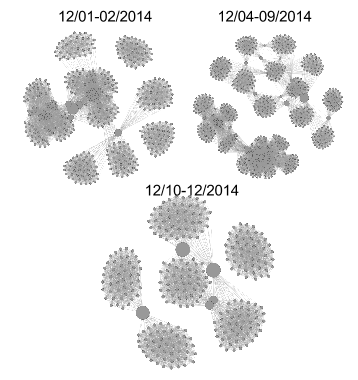
\includegraphics[width=0.6\textwidth]{hobbit-facebook-betweennes-centrality.png}
\caption{Highest betweenness centrality in the Fruchterman-Reingold layout for
the Facebook network of The Hobbit
\label{fig:hobbit-facebook-betweennes-centrality}}
\end{figure}
%
We can also notice that the "brokers" in the second network are smaller in size,
which means that less shortest paths pass through them than in the other
networks. This happens because there are more central nodes in the second
network than in the other two, so "the traffic" is split among them. Again, this
suggests that the Facebook page of the movie has become more popular during the
release dates in the US than in Europe.
%
\subsubsection{Communities in the Network}
Figure \ref{fig:hobbit-facebook-communities} shows the network colored based on
different communities and the users with the highest highest betweenness
centrality have been enlarged. These results have been yielded when determining
communities with a 1.0 modularity.
%
\begin{figure}
\centering
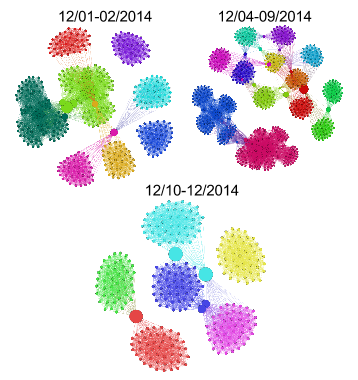
\includegraphics[width=0.6\textwidth]{hobbit-facebook-communities.png}
\caption{Communities in the Fruchterman-Reingold layout for the Facebook network
    of The Hobbit
\label{fig:hobbit-facebook-communities}}
\end{figure}
%
Just like the networks for the movie The Interview, the communities here are
very well defined and very well separated from one another. This time, however
we can see some differences between the three networks: for the first and
second graph, the communities have engulfed more than one post (which again
proves how popular the page was during this time frame); the third network,
however is smaller and the communities are only defined around single posts,
with a few brokers between them.
%
\subsubsection{Connected Components}
The connected components are displayed in figure \ref{fig:hobbit-facebook-cc}.
We can see that the first and the third network contain five, respectively three
connected components, whereas the second one contains only two.
%
\begin{figure}
\centering
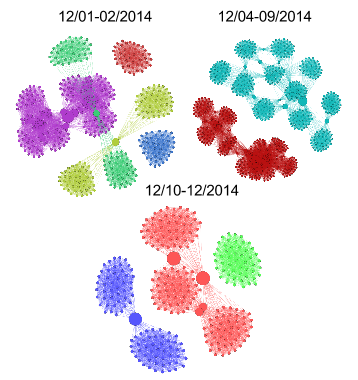
\includegraphics[width=0.6\textwidth]{hobbit-facebook-cc.png}
\caption{Connected components in the Fruchterman-Reingold layout for the
    Facebook network of The Hobbit
\label{fig:hobbit-facebook-cc}}
\end{figure}
%
\section{Conclusions}
The analysis of the four networks was based on data collected from the Facebook
and Twitter social web pages. However much we have strived, we could not import
all the data we desired to, due to the limitations of the existing tools and
APIs. Therefore, the graphs we have obtained are smaller than in reality. We
tried as much as possible to improve the quality of the data, by querying the
most popular tweets on Twitter and retrieving data from the release days on
Facebook.

There are several differences between the networks we have analysed and we have
highlighted these in the previous paragraphs. The most important would be: while
the Twitter networks are directed, the Facebook ones are undirected. In the
Twitter network, we have linked users to other users whose posts they have
retweeted, whereas in the Facebook network there is an edge between all the
users that were active around a post. Moreover, we have analysed the Facebook
network during certain periods of time, that have marked different release dates
of the two movies. Another difference would be that The Interview Twitter
network seems "younger" than The Hobbit's: the hubs and the authorities are not
yet well defined and the graph is rather sparse - there aren't many users who
have retweeted more than one post. Regarding the Facebook networks of the two
movies, The Hobbit has more users liking and commenting on their posts,
especially around the US release, while The Interview network is smaller and
doesn't change much in time.
%
\end{document}
